\documentclass{tufte-handout}
\usepackage{graphicx}
\graphicspath{ {./img/} }
\title{Introduction to Operating Systems}
\author{Andr\'es Ponce}

\begin{document}
\maketitle
\begin{abstract}

\section{Introduction}
An \textbf{operating system}(OS) is a piece of software that lies between the
hardware and software layer inside a computer. 
The OS helps the machine allocate resources to processes that require them.
\end{abstract}

The OS allocates resources to different processes on a computer. 
\subsection{Computer System Organization}
When we have an I/O request, the device controller will receive a signal to load 
and move the data to the CPU or main memory. When this process is done, the controller
will send a signal to the CPU informing of a successful completion of the transfer.

There are wother ways of triggering a system interrupt. Sometimes the program might
create an interrupt, known as a \textbf{software interrupt}. Other times, the 
hardware itself might create an interrupt. When this happens, there is a wire
connected to the CPU which is directly activated.

There are a couple useful distinctions:
\begin{itemize}
	\item Random Access: This type of memory allows any part of its data to be accessed
			without having to first access the other parts. This memory is 
			\textit{volatile}, which means it will be wiped clean next time the computers
			boot.
	\item Solid State: A solid state drive(SSD) uses solid state technology and removes
			any moving components from the drive. This allows for faster read speeds since
			we don't have to wait for the platter to spin in the correct decision 
			under the read/write head.
\end{itemize}

\begin{center}
	\begin{figure}
		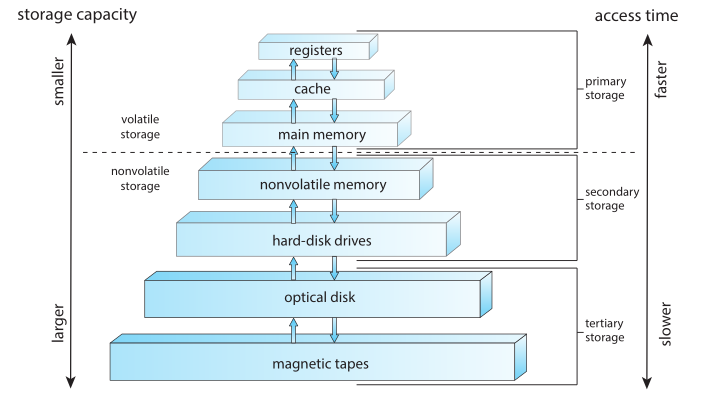
\includegraphics[scale=0.3]{mem_hierarchy}
		\caption{Memory hierarchy. As the speed of the memory increases, so does its
			cost. So we can only include a limited amount of very quick memory. Cache
			and registers usually are very limited and are located directly in the CPU.}
	\end{figure}
\end{center}


\subsection{Computer System Architecture}
In days past, the comptuer was able to run on a single \textbf{core}, which 
executed a general instruciton set needed by application programs. 
There could also be some smaller and different processors such as 
\textbf{controllers}.
\footnote{A \textbf{controller} is a type of device which handles taking information
from I/O devices and getting it to the CPU. A controller usually has its own buffer,
where it stores the data it is responsible for fetching before sending it to memory or 
CPU.}

However, recently there are multicore systems, which have more than one physical core.
This means that they can execute more than one instruction at at a time. 
However, it depends on whether there are any resources to allocate available.
These systems will usually share L2 cache, but L1 is local for each core. Since there
will be $N$ individual CPUs according to the comptuer, application programmers should
effectively use all the cores.

Why does continually adding more CPU cores not work \textit{ad infinitum}? There is 
an overhead performance penalty when trying to coordinate their loading. Also, once 
we add too many CPUs, the competition for the system bus might bottleneck performance.

\textbf{Blade servers} usually have multiple machines on the same chassis. 
\textbf{Clustered systems} are usually independent computers that share mostly storage.
They might be individual multicore systems that are interconnected to share storage.
Clustered systems are usually used in systems where we need the maximum reliability.
The advantage of having clustered systems is that we can monitor the performance of the
other nodes. We can assign one node in the cluster to monitor another one of the nodes.
If the observed node fails, we can set the monitoring node to take over the failed node's
operation, and report the error.

Some other types of netrowks might run on wide-area-networks and thus require to be 
connected over many miles. Software such as Oracle's database system might run on every 
onde in the network, as well as have a layer of software controlling other aspects of
resource allocation.

\subsection{Operating System Operations}
The first step the Operating System is responsible for is initializing the programs
that will run on the user's computer.
First, we load a \textbf{bootstrap} program, which is in charge of loading the operating
system into memory.

The kernel then runs and initializes I/O and starts other daemons. 
If there is nothing happening at the moment, then we wait 
for certain \textbf{interrupts}, which are the hardware's way of signalling events.
When a certain program is being executed, it is called a \textbf{process}. The CPU
has several programs in main memory at a given time, which leads to a better utilization
of the of the CPU. 
This is because the CPU might finish a program and will have to wait while the next 
one is loaded into memory. Also, the CPU might be idle while waiting for an I/O operation.
If the CPU did not have another program to execute in the meantime, the CPU would idle.

\subsection{Dual-Mode Operation}
We also need to differentiate between user programs that are executing and actual 
OS code that is running. We need this to ensure that malicious user programs cannot
affect the way the OS runs. The two modes are: \textbf{user mode} and \textbf{kernel mode}.
We distinguis them by using a \textbf{mode bit} directly in the hardware. When the OS 
first loads, it does so in kernel mode, and when it's time to execute a user program,
we switch the bit to user mode.

\subsection{Resource Management}
We remember that the OS is the main reource manager in a system. This means that when
a process requires some memory resources, the CPU will allcoate those resources and then 
reclaim them when the process is over.

\textbf{Memory management} requires us to efficiently use the main memory. When a program
is executed, it first has to be loaded into main memory. It uses a direct address to fetch
the instruction to execute next. The OS can decide when the information needs to move in
and out of main memory and how much space the process requires.

The computer stores information in a the basic logical storage unit called a \textbf{file}.
Files are then stored on secondary and tertiary storage, and can take either textual
or binary form.

\end{document}
